\documentclass[1p]{elsarticle_modified}
%\bibliographystyle{elsarticle-num}

%\usepackage[colorlinks]{hyperref}
%\usepackage{abbrmath_seonhwa} %\Abb, \Ascr, \Acal ,\Abf, \Afrak
\usepackage{amsfonts}
\usepackage{amssymb}
\usepackage{amsmath}
\usepackage{amsthm}
\usepackage{scalefnt}
\usepackage{amsbsy}
\usepackage{kotex}
\usepackage{caption}
\usepackage{subfig}
\usepackage{color}
\usepackage{graphicx}
\usepackage{xcolor} %% white, black, red, green, blue, cyan, magenta, yellow
\usepackage{float}
\usepackage{setspace}
\usepackage{hyperref}

\usepackage{tikz}
\usetikzlibrary{arrows}

\usepackage{multirow}
\usepackage{array} % fixed length table
\usepackage{hhline}

%%%%%%%%%%%%%%%%%%%%%
\makeatletter
\renewcommand*\env@matrix[1][\arraystretch]{%
	\edef\arraystretch{#1}%
	\hskip -\arraycolsep
	\let\@ifnextchar\new@ifnextchar
	\array{*\c@MaxMatrixCols c}}
\makeatother %https://tex.stackexchange.com/questions/14071/how-can-i-increase-the-line-spacing-in-a-matrix
%%%%%%%%%%%%%%%

\usepackage[normalem]{ulem}

\newcommand{\msout}[1]{\ifmmode\text{\sout{\ensuremath{#1}}}\else\sout{#1}\fi}
%SOURCE: \msout is \stkout macro in https://tex.stackexchange.com/questions/20609/strikeout-in-math-mode

\newcommand{\cancel}[1]{
	\ifmmode
	{\color{red}\msout{#1}}
	\else
	{\color{red}\sout{#1}}
	\fi
}

\newcommand{\add}[1]{
	{\color{blue}\uwave{#1}}
}

\newcommand{\replace}[2]{
	\ifmmode
	{\color{red}\msout{#1}}{\color{blue}\uwave{#2}}
	\else
	{\color{red}\sout{#1}}{\color{blue}\uwave{#2}}
	\fi
}

\newcommand{\Sol}{\mathcal{S}} %segment
\newcommand{\D}{D} %diagram
\newcommand{\A}{\mathcal{A}} %arc


%%%%%%%%%%%%%%%%%%%%%%%%%%%%%5 test

\def\sl{\operatorname{\textup{SL}}(2,\Cbb)}
\def\psl{\operatorname{\textup{PSL}}(2,\Cbb)}
\def\quan{\mkern 1mu \triangleright \mkern 1mu}

\theoremstyle{definition}
\newtheorem{thm}{Theorem}[section]
\newtheorem{prop}[thm]{Proposition}
\newtheorem{lem}[thm]{Lemma}
\newtheorem{ques}[thm]{Question}
\newtheorem{cor}[thm]{Corollary}
\newtheorem{defn}[thm]{Definition}
\newtheorem{exam}[thm]{Example}
\newtheorem{rmk}[thm]{Remark}
\newtheorem{alg}[thm]{Algorithm}

\newcommand{\I}{\sqrt{-1}}
\begin{document}

%\begin{frontmatter}
%
%\title{Boundary parabolic representations of knots up to 8 crossings}
%
%%% Group authors per affiliation:
%\author{Yunhi Cho} 
%\address{Department of Mathematics, University of Seoul, Seoul, Korea}
%\ead{yhcho@uos.ac.kr}
%
%
%\author{Seonhwa Kim} %\fnref{s_kim}}
%\address{Center for Geometry and Physics, Institute for Basic Science, Pohang, 37673, Korea}
%\ead{ryeona17@ibs.re.kr}
%
%\author{Hyuk Kim}
%\address{Department of Mathematical Sciences, Seoul National University, Seoul 08826, Korea}
%\ead{hyukkim@snu.ac.kr}
%
%\author{Seokbeom Yoon}
%\address{Department of Mathematical Sciences, Seoul National University, Seoul, 08826,  Korea}
%\ead{sbyoon15@snu.ac.kr}
%
%\begin{abstract}
%We find all boundary parabolic representation of knots up to 8 crossings.
%
%\end{abstract}
%\begin{keyword}
%    \MSC[2010] 57M25 
%\end{keyword}
%
%\end{frontmatter}

%\linenumbers
%\tableofcontents
%
\newcommand\colored[1]{\textcolor{white}{\rule[-0.35ex]{0.8em}{1.4ex}}\kern-0.8em\color{red} #1}%
%\newcommand\colored[1]{\textcolor{white}{ #1}\kern-2.17ex	\textcolor{white}{ #1}\kern-1.81ex	\textcolor{white}{ #1}\kern-2.15ex\color{red}#1	}

{\Large $\underline{12a_{1032}~(K12a_{1032})}$}

\setlength{\tabcolsep}{10pt}
\renewcommand{\arraystretch}{1.6}
\vspace{1cm}\begin{tabular}{m{100pt}>{\centering\arraybackslash}m{274pt}}
\multirow{5}{120pt}{
	\centering
	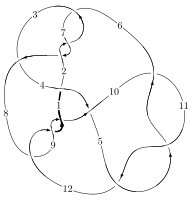
\includegraphics[width=112pt]{../../../GIT/diagram.site/Diagrams/png/1833_12a_1032.png}\\
\ \ \ A knot diagram\footnotemark}&
\allowdisplaybreaks
\textbf{Linearized knot diagam} \\
\cline{2-2}
 &
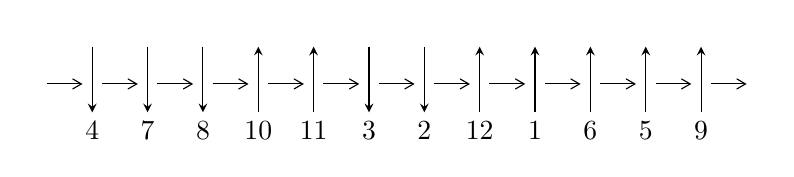
\begin{tikzpicture}[x=20pt, y=17pt]
	% nodes
	\node (C0) at (0, 0) {};
	\node (C1) at (1, 0) {};
	\node (C1U) at (1, +1) {};
	\node (C1D) at (1, -1) {4};

	\node (C2) at (2, 0) {};
	\node (C2U) at (2, +1) {};
	\node (C2D) at (2, -1) {7};

	\node (C3) at (3, 0) {};
	\node (C3U) at (3, +1) {};
	\node (C3D) at (3, -1) {8};

	\node (C4) at (4, 0) {};
	\node (C4U) at (4, +1) {};
	\node (C4D) at (4, -1) {10};

	\node (C5) at (5, 0) {};
	\node (C5U) at (5, +1) {};
	\node (C5D) at (5, -1) {11};

	\node (C6) at (6, 0) {};
	\node (C6U) at (6, +1) {};
	\node (C6D) at (6, -1) {3};

	\node (C7) at (7, 0) {};
	\node (C7U) at (7, +1) {};
	\node (C7D) at (7, -1) {2};

	\node (C8) at (8, 0) {};
	\node (C8U) at (8, +1) {};
	\node (C8D) at (8, -1) {12};

	\node (C9) at (9, 0) {};
	\node (C9U) at (9, +1) {};
	\node (C9D) at (9, -1) {1};

	\node (C10) at (10, 0) {};
	\node (C10U) at (10, +1) {};
	\node (C10D) at (10, -1) {6};

	\node (C11) at (11, 0) {};
	\node (C11U) at (11, +1) {};
	\node (C11D) at (11, -1) {5};

	\node (C12) at (12, 0) {};
	\node (C12U) at (12, +1) {};
	\node (C12D) at (12, -1) {9};
	\node (C13) at (13, 0) {};

	% arrows
	\draw[->,>={angle 60}]
	(C0) edge (C1) (C1) edge (C2) (C2) edge (C3) (C3) edge (C4) (C4) edge (C5) (C5) edge (C6) (C6) edge (C7) (C7) edge (C8) (C8) edge (C9) (C9) edge (C10) (C10) edge (C11) (C11) edge (C12) (C12) edge (C13) ;	\draw[->,>=stealth]
	(C1U) edge (C1D) (C2U) edge (C2D) (C3U) edge (C3D) (C4D) edge (C4U) (C5D) edge (C5U) (C6U) edge (C6D) (C7U) edge (C7D) (C8D) edge (C8U) (C9D) edge (C9U) (C10D) edge (C10U) (C11D) edge (C11U) (C12D) edge (C12U) ;
	\end{tikzpicture} \\
\hhline{~~} \\& 
\textbf{Solving Sequence} \\ \cline{2-2} 
 &
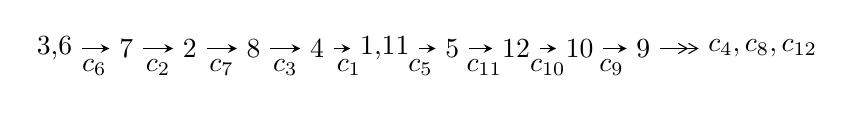
\begin{tikzpicture}[x=23pt, y=7pt]
	% node
	\node (A0) at (-1/8, 0) {3,6};
	\node (A1) at (1, 0) {7};
	\node (A2) at (2, 0) {2};
	\node (A3) at (3, 0) {8};
	\node (A4) at (4, 0) {4};
	\node (A5) at (81/16, 0) {1,11};
	\node (A6) at (49/8, 0) {5};
	\node (A7) at (57/8, 0) {12};
	\node (A8) at (65/8, 0) {10};
	\node (A9) at (73/8, 0) {9};
	\node (C1) at (1/2, -1) {$c_{6}$};
	\node (C2) at (3/2, -1) {$c_{2}$};
	\node (C3) at (5/2, -1) {$c_{7}$};
	\node (C4) at (7/2, -1) {$c_{3}$};
	\node (C5) at (9/2, -1) {$c_{1}$};
	\node (C6) at (45/8, -1) {$c_{5}$};
	\node (C7) at (53/8, -1) {$c_{11}$};
	\node (C8) at (61/8, -1) {$c_{10}$};
	\node (C9) at (69/8, -1) {$c_{9}$};
	\node (A10) at (11, 0) {$c_{4},c_{8},c_{12}$};

	% edge
	\draw[->,>=stealth]	
	(A0) edge (A1) (A1) edge (A2) (A2) edge (A3) (A3) edge (A4) (A4) edge (A5) (A5) edge (A6) (A6) edge (A7) (A7) edge (A8) (A8) edge (A9) ;
	\draw[->>,>={angle 60}]	
	(A9) edge (A10);
\end{tikzpicture} \\ 

\end{tabular} \\

\footnotetext{
The image of knot diagram is generated by the software ``\textbf{Draw programme}" developed by Andrew Bartholomew(\url{http://www.layer8.co.uk/maths/draw/index.htm\#Running-draw}), where we modified some parts for our purpose(\url{https://github.com/CATsTAILs/LinksPainter}).
}\phantom \\ \newline 
\centering \textbf{Ideals for irreducible components\footnotemark of $X_{\text{par}}$} 
 
\begin{align*}
I^u_{1}&=\langle 
-5.13488\times10^{22} u^{77}+6.96847\times10^{23} u^{76}+\cdots+1.38959\times10^{24} b+9.38953\times10^{23},\\
\phantom{I^u_{1}}&\phantom{= \langle  }1.56764\times10^{24} u^{77}+2.54331\times10^{24} u^{76}+\cdots+4.16876\times10^{24} a-1.01501\times10^{25},\;u^{78}+2 u^{77}+\cdots-3 u-3\rangle \\
I^u_{2}&=\langle 
b,\;- u^2+a-1,\;u^3+u^2+2 u+1\rangle \\
I^u_{3}&=\langle 
u^2 a-2 a u+3 u^2+5 b- a- u+2,\;-2 u^2 a+a^2+9 u^2-2 a-7 u+18,\;u^3- u^2+2 u-1\rangle \\
\\
\end{align*}
\raggedright * 3 irreducible components of $\dim_{\mathbb{C}}=0$, with total 87 representations.\\
\footnotetext{All coefficients of polynomials are rational numbers. But the coefficients are sometimes approximated in decimal forms when there is not enough margin.}
\newpage
\renewcommand{\arraystretch}{1}
\centering \section*{I. $I^u_{1}= \langle -5.13\times10^{22} u^{77}+6.97\times10^{23} u^{76}+\cdots+1.39\times10^{24} b+9.39\times10^{23},\;1.57\times10^{24} u^{77}+2.54\times10^{24} u^{76}+\cdots+4.17\times10^{24} a-1.02\times10^{25},\;u^{78}+2 u^{77}+\cdots-3 u-3 \rangle$}
\flushleft \textbf{(i) Arc colorings}\\
\begin{tabular}{m{7pt} m{180pt} m{7pt} m{180pt} }
\flushright $a_{3}=$&$\begin{pmatrix}0\\u\end{pmatrix}$ \\
\flushright $a_{6}=$&$\begin{pmatrix}1\\0\end{pmatrix}$ \\
\flushright $a_{7}=$&$\begin{pmatrix}1\\u^2\end{pmatrix}$ \\
\flushright $a_{2}=$&$\begin{pmatrix}u\\u^3+u\end{pmatrix}$ \\
\flushright $a_{8}=$&$\begin{pmatrix}u^2+1\\u^4+2 u^2\end{pmatrix}$ \\
\flushright $a_{4}=$&$\begin{pmatrix}- u^5-2 u^3- u\\- u^7-3 u^5-2 u^3+u\end{pmatrix}$ \\
\flushright $a_{1}=$&$\begin{pmatrix}u^9+4 u^7+5 u^5+2 u^3+u\\u^{11}+5 u^9+8 u^7+3 u^5- u^3+u\end{pmatrix}$ \\
\flushright $a_{11}=$&$\begin{pmatrix}-0.376045 u^{77}-0.610088 u^{76}+\cdots+1.32049 u+2.43481\\0.0369526 u^{77}-0.501478 u^{76}+\cdots+0.585143 u-0.675707\end{pmatrix}$ \\
\flushright $a_{5}=$&$\begin{pmatrix}1.26294 u^{77}+2.25066 u^{76}+\cdots-2.84986 u-1.41015\\-0.307268 u^{77}-0.831343 u^{76}+\cdots+3.63374 u+0.384719\end{pmatrix}$ \\
\flushright $a_{12}=$&$\begin{pmatrix}0.259199 u^{77}+0.274703 u^{76}+\cdots+2.57149 u-0.449948\\0.0447472 u^{77}+0.572456 u^{76}+\cdots-1.87435 u+0.827634\end{pmatrix}$ \\
\flushright $a_{10}=$&$\begin{pmatrix}-0.412998 u^{77}-0.108610 u^{76}+\cdots+0.735348 u+3.11052\\0.0369526 u^{77}-0.501478 u^{76}+\cdots+0.585143 u-0.675707\end{pmatrix}$ \\
\flushright $a_{9}=$&$\begin{pmatrix}-0.454996 u^{77}-0.635848 u^{76}+\cdots+2.02928 u+2.79107\\-0.00885144 u^{77}-0.531385 u^{76}+\cdots+0.546815 u-0.805065\end{pmatrix}$\\&\end{tabular}
\flushleft \textbf{(ii) Obstruction class $= -1$}\\~\\
\flushleft \textbf{(iii) Cusp Shapes $= \frac{2155115887218372860035718}{694792694815903195651135} u^{77}+\frac{4180801602356197336101919}{694792694815903195651135} u^{76}+\cdots+\frac{9214508540967252021234482}{694792694815903195651135} u-\frac{2286501097268875425262962}{694792694815903195651135}$}\\~\\
\newpage\renewcommand{\arraystretch}{1}
\flushleft \textbf{(iv) u-Polynomials at the component}\newline \\
\begin{tabular}{m{50pt}|m{274pt}}
Crossings & \hspace{64pt}u-Polynomials at each crossing \\
\hline $$\begin{aligned}c_{1}\end{aligned}$$&$\begin{aligned}
&u^{78}-16 u^{77}+\cdots-227379 u+30627
\end{aligned}$\\
\hline $$\begin{aligned}c_{2},c_{6},c_{7}\end{aligned}$$&$\begin{aligned}
&u^{78}+2 u^{77}+\cdots-3 u-3
\end{aligned}$\\
\hline $$\begin{aligned}c_{3}\end{aligned}$$&$\begin{aligned}
&u^{78}-2 u^{77}+\cdots-1479 u-867
\end{aligned}$\\
\hline $$\begin{aligned}c_{4}\end{aligned}$$&$\begin{aligned}
&u^{78}- u^{77}+\cdots+4032 u+3112
\end{aligned}$\\
\hline $$\begin{aligned}c_{5},c_{10},c_{11}\end{aligned}$$&$\begin{aligned}
&u^{78}+u^{77}+\cdots-32 u^2+8
\end{aligned}$\\
\hline $$\begin{aligned}c_{8},c_{9},c_{12}\end{aligned}$$&$\begin{aligned}
&u^{78}-4 u^{77}+\cdots-108 u-17
\end{aligned}$\\
\hline
\end{tabular}\\~\\
\newpage\renewcommand{\arraystretch}{1}
\flushleft \textbf{(v) Riley Polynomials at the component}\newline \\
\begin{tabular}{m{50pt}|m{274pt}}
Crossings & \hspace{64pt}Riley Polynomials at each crossing \\
\hline $$\begin{aligned}c_{1}\end{aligned}$$&$\begin{aligned}
&y^{78}+32 y^{77}+\cdots+2934785691 y+938013129
\end{aligned}$\\
\hline $$\begin{aligned}c_{2},c_{6},c_{7}\end{aligned}$$&$\begin{aligned}
&y^{78}+72 y^{77}+\cdots-129 y+9
\end{aligned}$\\
\hline $$\begin{aligned}c_{3}\end{aligned}$$&$\begin{aligned}
&y^{78}+8 y^{77}+\cdots+5081487 y+751689
\end{aligned}$\\
\hline $$\begin{aligned}c_{4}\end{aligned}$$&$\begin{aligned}
&y^{78}-13 y^{77}+\cdots-77550976 y+9684544
\end{aligned}$\\
\hline $$\begin{aligned}c_{5},c_{10},c_{11}\end{aligned}$$&$\begin{aligned}
&y^{78}+71 y^{77}+\cdots-512 y+64
\end{aligned}$\\
\hline $$\begin{aligned}c_{8},c_{9},c_{12}\end{aligned}$$&$\begin{aligned}
&y^{78}-74 y^{77}+\cdots+5540 y+289
\end{aligned}$\\
\hline
\end{tabular}\\~\\
\newpage\flushleft \textbf{(vi) Complex Volumes and Cusp Shapes}
$$\begin{array}{c|c|c}  
\text{Solutions to }I^u_{1}& \I (\text{vol} + \sqrt{-1}CS) & \text{Cusp shape}\\
 \hline 
\begin{aligned}
u &= \phantom{-}0.192957 + 1.111600 I \\
a &= \phantom{-}1.19779 + 2.02532 I \\
b &= -0.168435 + 1.396140 I\end{aligned}
 & -3.81969 - 3.89814 I & \phantom{-0.000000 } 0 \\ \hline\begin{aligned}
u &= \phantom{-}0.192957 - 1.111600 I \\
a &= \phantom{-}1.19779 - 2.02532 I \\
b &= -0.168435 - 1.396140 I\end{aligned}
 & -3.81969 + 3.89814 I & \phantom{-0.000000 } 0 \\ \hline\begin{aligned}
u &= \phantom{-}0.320913 + 1.119940 I \\
a &= -0.94949 - 2.09661 I \\
b &= \phantom{-}0.262940 - 1.340440 I\end{aligned}
 & \phantom{-}1.05376 - 7.02286 I & \phantom{-0.000000 } 0 \\ \hline\begin{aligned}
u &= \phantom{-}0.320913 - 1.119940 I \\
a &= -0.94949 + 2.09661 I \\
b &= \phantom{-}0.262940 + 1.340440 I\end{aligned}
 & \phantom{-}1.05376 + 7.02286 I & \phantom{-0.000000 } 0 \\ \hline\begin{aligned}
u &= -0.473389 + 0.686908 I \\
a &= \phantom{-}0.08281 - 1.56208 I \\
b &= \phantom{-}0.33298 - 1.38387 I\end{aligned}
 & \phantom{-}2.38668 - 7.05623 I & \phantom{-}4.04957 + 2.76916 I \\ \hline\begin{aligned}
u &= -0.473389 - 0.686908 I \\
a &= \phantom{-}0.08281 + 1.56208 I \\
b &= \phantom{-}0.33298 + 1.38387 I\end{aligned}
 & \phantom{-}2.38668 + 7.05623 I & \phantom{-}4.04957 - 2.76916 I \\ \hline\begin{aligned}
u &= -0.079678 + 1.178770 I \\
a &= \phantom{-}0.286269 - 0.635203 I \\
b &= -0.475807 - 0.361911 I\end{aligned}
 & \phantom{-}1.71847 + 1.56145 I & \phantom{-0.000000 } 0 \\ \hline\begin{aligned}
u &= -0.079678 - 1.178770 I \\
a &= \phantom{-}0.286269 + 0.635203 I \\
b &= -0.475807 + 0.361911 I\end{aligned}
 & \phantom{-}1.71847 - 1.56145 I & \phantom{-0.000000 } 0 \\ \hline\begin{aligned}
u &= -0.747048 + 0.324353 I \\
a &= \phantom{-}1.52805 - 2.73924 I \\
b &= -0.33672 - 1.41782 I\end{aligned}
 & \phantom{-}1.11303 + 11.32630 I & \phantom{-}1.74011 - 7.84897 I \\ \hline\begin{aligned}
u &= -0.747048 - 0.324353 I \\
a &= \phantom{-}1.52805 + 2.73924 I \\
b &= -0.33672 + 1.41782 I\end{aligned}
 & \phantom{-}1.11303 - 11.32630 I & \phantom{-}1.74011 + 7.84897 I\\
 \hline 
 \end{array}$$\newpage$$\begin{array}{c|c|c}  
\text{Solutions to }I^u_{1}& \I (\text{vol} + \sqrt{-1}CS) & \text{Cusp shape}\\
 \hline 
\begin{aligned}
u &= \phantom{-}0.030969 + 1.197970 I \\
a &= -1.68028 - 1.82896 I \\
b &= \phantom{-}0.12649 - 1.43914 I\end{aligned}
 & -1.033450 - 0.444387 I & \phantom{-0.000000 } 0 \\ \hline\begin{aligned}
u &= \phantom{-}0.030969 - 1.197970 I \\
a &= -1.68028 + 1.82896 I \\
b &= \phantom{-}0.12649 + 1.43914 I\end{aligned}
 & -1.033450 + 0.444387 I & \phantom{-0.000000 } 0 \\ \hline\begin{aligned}
u &= \phantom{-}0.717522 + 0.354101 I \\
a &= -0.151776 + 1.187950 I \\
b &= -0.818337 + 0.262522 I\end{aligned}
 & \phantom{-}6.45672 - 7.14735 I & \phantom{-}6.13824 + 6.79892 I \\ \hline\begin{aligned}
u &= \phantom{-}0.717522 - 0.354101 I \\
a &= -0.151776 - 1.187950 I \\
b &= -0.818337 - 0.262522 I\end{aligned}
 & \phantom{-}6.45672 + 7.14735 I & \phantom{-}6.13824 - 6.79892 I \\ \hline\begin{aligned}
u &= \phantom{-}0.506406 + 0.609564 I \\
a &= \phantom{-}0.129930 - 0.090005 I \\
b &= \phantom{-}0.805112 + 0.201005 I\end{aligned}
 & \phantom{-}7.40344 + 2.95162 I & \phantom{-}8.38298 - 0.93021 I \\ \hline\begin{aligned}
u &= \phantom{-}0.506406 - 0.609564 I \\
a &= \phantom{-}0.129930 + 0.090005 I \\
b &= \phantom{-}0.805112 - 0.201005 I\end{aligned}
 & \phantom{-}7.40344 - 2.95162 I & \phantom{-}8.38298 + 0.93021 I \\ \hline\begin{aligned}
u &= \phantom{-}0.771376 + 0.082944 I \\
a &= -0.44711 - 3.10641 I \\
b &= -0.231533 - 1.297700 I\end{aligned}
 & -2.11544 + 3.03018 I & \phantom{-}0.27772 - 2.58777 I \\ \hline\begin{aligned}
u &= \phantom{-}0.771376 - 0.082944 I \\
a &= -0.44711 + 3.10641 I \\
b &= -0.231533 + 1.297700 I\end{aligned}
 & -2.11544 - 3.03018 I & \phantom{-}0.27772 + 2.58777 I \\ \hline\begin{aligned}
u &= -0.290042 + 1.206290 I \\
a &= \phantom{-}0.139811 + 0.526105 I \\
b &= \phantom{-}0.621955 + 0.111558 I\end{aligned}
 & \phantom{-}5.66191 + 3.76271 I & \phantom{-0.000000 } 0 \\ \hline\begin{aligned}
u &= -0.290042 - 1.206290 I \\
a &= \phantom{-}0.139811 - 0.526105 I \\
b &= \phantom{-}0.621955 - 0.111558 I\end{aligned}
 & \phantom{-}5.66191 - 3.76271 I & \phantom{-0.000000 } 0\\
 \hline 
 \end{array}$$\newpage$$\begin{array}{c|c|c}  
\text{Solutions to }I^u_{1}& \I (\text{vol} + \sqrt{-1}CS) & \text{Cusp shape}\\
 \hline 
\begin{aligned}
u &= -0.655866 + 0.382150 I \\
a &= -0.807968 + 0.893907 I \\
b &= -0.474927 + 0.866530 I\end{aligned}
 & \phantom{-}4.52645 + 2.56217 I & \phantom{-}4.50484 - 2.46419 I \\ \hline\begin{aligned}
u &= -0.655866 - 0.382150 I \\
a &= -0.807968 - 0.893907 I \\
b &= -0.474927 - 0.866530 I\end{aligned}
 & \phantom{-}4.52645 - 2.56217 I & \phantom{-}4.50484 + 2.46419 I \\ \hline\begin{aligned}
u &= -0.693288 + 0.304422 I \\
a &= -1.95436 + 2.45062 I \\
b &= \phantom{-}0.272595 + 1.371760 I\end{aligned}
 & -4.48416 + 7.09115 I & -2.04061 - 7.55095 I \\ \hline\begin{aligned}
u &= -0.693288 - 0.304422 I \\
a &= -1.95436 - 2.45062 I \\
b &= \phantom{-}0.272595 - 1.371760 I\end{aligned}
 & -4.48416 - 7.09115 I & -2.04061 + 7.55095 I \\ \hline\begin{aligned}
u &= -0.550306 + 0.508147 I \\
a &= -0.71523 + 1.43481 I \\
b &= \phantom{-}0.411750 + 0.974001 I\end{aligned}
 & \phantom{-}5.00598 + 1.43831 I & \phantom{-}5.56279 - 3.99254 I \\ \hline\begin{aligned}
u &= -0.550306 - 0.508147 I \\
a &= -0.71523 - 1.43481 I \\
b &= \phantom{-}0.411750 - 0.974001 I\end{aligned}
 & \phantom{-}5.00598 - 1.43831 I & \phantom{-}5.56279 + 3.99254 I \\ \hline\begin{aligned}
u &= -0.742831\phantom{ +0.000000I} \\
a &= -0.898304\phantom{ +0.000000I} \\
b &= -0.609293\phantom{ +0.000000I}\end{aligned}
 & \phantom{-}1.96168\phantom{ +0.000000I} & \phantom{-}5.99100\phantom{ +0.000000I} \\ \hline\begin{aligned}
u &= \phantom{-}0.088144 + 1.269300 I \\
a &= -0.813357 + 0.841995 I \\
b &= \phantom{-}0.443490 + 0.349624 I\end{aligned}
 & \phantom{-}4.80145 - 1.58760 I & \phantom{-0.000000 } 0 \\ \hline\begin{aligned}
u &= \phantom{-}0.088144 - 1.269300 I \\
a &= -0.813357 - 0.841995 I \\
b &= \phantom{-}0.443490 - 0.349624 I\end{aligned}
 & \phantom{-}4.80145 + 1.58760 I & \phantom{-0.000000 } 0 \\ \hline\begin{aligned}
u &= \phantom{-}0.625985 + 0.307354 I \\
a &= -0.280689 - 1.134010 I \\
b &= \phantom{-}0.662399 - 0.196150 I\end{aligned}
 & \phantom{-}0.48579 - 3.66760 I & \phantom{-}3.12377 + 7.79182 I\\
 \hline 
 \end{array}$$\newpage$$\begin{array}{c|c|c}  
\text{Solutions to }I^u_{1}& \I (\text{vol} + \sqrt{-1}CS) & \text{Cusp shape}\\
 \hline 
\begin{aligned}
u &= \phantom{-}0.625985 - 0.307354 I \\
a &= -0.280689 + 1.134010 I \\
b &= \phantom{-}0.662399 + 0.196150 I\end{aligned}
 & \phantom{-}0.48579 + 3.66760 I & \phantom{-}3.12377 - 7.79182 I \\ \hline\begin{aligned}
u &= -0.374022 + 0.584619 I \\
a &= \phantom{-}0.281584 + 1.126590 I \\
b &= -0.229914 + 1.337150 I\end{aligned}
 & -3.29505 - 3.31684 I & \phantom{-}0.37580 + 2.22795 I \\ \hline\begin{aligned}
u &= -0.374022 - 0.584619 I \\
a &= \phantom{-}0.281584 - 1.126590 I \\
b &= -0.229914 - 1.337150 I\end{aligned}
 & -3.29505 + 3.31684 I & \phantom{-}0.37580 - 2.22795 I \\ \hline\begin{aligned}
u &= \phantom{-}0.671062 + 0.114541 I \\
a &= \phantom{-}0.46437 + 3.46215 I \\
b &= \phantom{-}0.109881 + 1.399800 I\end{aligned}
 & -6.76019 + 0.61306 I & -7.17730 + 0.24747 I \\ \hline\begin{aligned}
u &= \phantom{-}0.671062 - 0.114541 I \\
a &= \phantom{-}0.46437 - 3.46215 I \\
b &= \phantom{-}0.109881 - 1.399800 I\end{aligned}
 & -6.76019 - 0.61306 I & -7.17730 - 0.24747 I \\ \hline\begin{aligned}
u &= -0.607811 + 0.306243 I \\
a &= \phantom{-}2.18924 - 1.51724 I \\
b &= -0.195606 - 1.287310 I\end{aligned}
 & -2.60345 + 2.27614 I & \phantom{-}0.75235 - 3.81852 I \\ \hline\begin{aligned}
u &= -0.607811 - 0.306243 I \\
a &= \phantom{-}2.18924 + 1.51724 I \\
b &= -0.195606 + 1.287310 I\end{aligned}
 & -2.60345 - 2.27614 I & \phantom{-}0.75235 + 3.81852 I \\ \hline\begin{aligned}
u &= \phantom{-}0.321608 + 1.293240 I \\
a &= \phantom{-}0.86084 + 1.56808 I \\
b &= \phantom{-}0.198523 + 1.256840 I\end{aligned}
 & \phantom{-}2.16962 - 0.91182 I & \phantom{-0.000000 } 0 \\ \hline\begin{aligned}
u &= \phantom{-}0.321608 - 1.293240 I \\
a &= \phantom{-}0.86084 - 1.56808 I \\
b &= \phantom{-}0.198523 - 1.256840 I\end{aligned}
 & \phantom{-}2.16962 + 0.91182 I & \phantom{-0.000000 } 0 \\ \hline\begin{aligned}
u &= \phantom{-}0.251582 + 1.328590 I \\
a &= -0.98352 - 1.56576 I \\
b &= -0.07092 - 1.41475 I\end{aligned}
 & -2.23585 - 2.71517 I & \phantom{-0.000000 } 0\\
 \hline 
 \end{array}$$\newpage$$\begin{array}{c|c|c}  
\text{Solutions to }I^u_{1}& \I (\text{vol} + \sqrt{-1}CS) & \text{Cusp shape}\\
 \hline 
\begin{aligned}
u &= \phantom{-}0.251582 - 1.328590 I \\
a &= -0.98352 + 1.56576 I \\
b &= -0.07092 + 1.41475 I\end{aligned}
 & -2.23585 + 2.71517 I & \phantom{-0.000000 } 0 \\ \hline\begin{aligned}
u &= -0.202356 + 1.364250 I \\
a &= -0.368264 - 0.065956 I \\
b &= -0.067803 + 0.563459 I\end{aligned}
 & \phantom{-}3.79199 + 3.49836 I & \phantom{-0.000000 } 0 \\ \hline\begin{aligned}
u &= -0.202356 - 1.364250 I \\
a &= -0.368264 + 0.065956 I \\
b &= -0.067803 - 0.563459 I\end{aligned}
 & \phantom{-}3.79199 - 3.49836 I & \phantom{-0.000000 } 0 \\ \hline\begin{aligned}
u &= \phantom{-}0.546679 + 0.273991 I \\
a &= -1.04542 - 3.63991 I \\
b &= -0.04558 - 1.51756 I\end{aligned}
 & -3.36178 - 1.38887 I & \phantom{-}2.35610 + 5.10659 I \\ \hline\begin{aligned}
u &= \phantom{-}0.546679 - 0.273991 I \\
a &= -1.04542 + 3.63991 I \\
b &= -0.04558 + 1.51756 I\end{aligned}
 & -3.36178 + 1.38887 I & \phantom{-}2.35610 - 5.10659 I \\ \hline\begin{aligned}
u &= -0.435351 + 0.389359 I \\
a &= \phantom{-}0.491782 - 0.204328 I \\
b &= \phantom{-}0.084335 - 1.208670 I\end{aligned}
 & -2.01640 + 0.97897 I & \phantom{-}2.34600 - 4.48200 I \\ \hline\begin{aligned}
u &= -0.435351 - 0.389359 I \\
a &= \phantom{-}0.491782 + 0.204328 I \\
b &= \phantom{-}0.084335 + 1.208670 I\end{aligned}
 & -2.01640 - 0.97897 I & \phantom{-}2.34600 + 4.48200 I \\ \hline\begin{aligned}
u &= -0.18432 + 1.40986 I \\
a &= -0.225592 - 0.553357 I \\
b &= -0.152154 + 1.055850 I\end{aligned}
 & \phantom{-}3.63556 + 3.32279 I & \phantom{-0.000000 } 0 \\ \hline\begin{aligned}
u &= -0.18432 - 1.40986 I \\
a &= -0.225592 + 0.553357 I \\
b &= -0.152154 - 1.055850 I\end{aligned}
 & \phantom{-}3.63556 - 3.32279 I & \phantom{-0.000000 } 0 \\ \hline\begin{aligned}
u &= \phantom{-}0.21945 + 1.40861 I \\
a &= \phantom{-}0.96270 + 1.46545 I \\
b &= \phantom{-}0.04850 + 1.56203 I\end{aligned}
 & \phantom{-}2.03927 - 4.24747 I & \phantom{-0.000000 } 0\\
 \hline 
 \end{array}$$\newpage$$\begin{array}{c|c|c}  
\text{Solutions to }I^u_{1}& \I (\text{vol} + \sqrt{-1}CS) & \text{Cusp shape}\\
 \hline 
\begin{aligned}
u &= \phantom{-}0.21945 - 1.40861 I \\
a &= \phantom{-}0.96270 - 1.46545 I \\
b &= \phantom{-}0.04850 - 1.56203 I\end{aligned}
 & \phantom{-}2.03927 + 4.24747 I & \phantom{-0.000000 } 0 \\ \hline\begin{aligned}
u &= -0.548507 + 0.166008 I \\
a &= \phantom{-}0.530033 - 0.629098 I \\
b &= \phantom{-}0.218693 - 0.435531 I\end{aligned}
 & -1.097180 + 0.763622 I & -4.24671 - 2.11774 I \\ \hline\begin{aligned}
u &= -0.548507 - 0.166008 I \\
a &= \phantom{-}0.530033 + 0.629098 I \\
b &= \phantom{-}0.218693 + 0.435531 I\end{aligned}
 & -1.097180 - 0.763622 I & -4.24671 + 2.11774 I \\ \hline\begin{aligned}
u &= \phantom{-}0.18767 + 1.41646 I \\
a &= -1.098180 - 0.416185 I \\
b &= \phantom{-}0.692130 + 0.004260 I\end{aligned}
 & \phantom{-}6.83413 - 1.96589 I & \phantom{-0.000000 } 0 \\ \hline\begin{aligned}
u &= \phantom{-}0.18767 - 1.41646 I \\
a &= -1.098180 + 0.416185 I \\
b &= \phantom{-}0.692130 - 0.004260 I\end{aligned}
 & \phantom{-}6.83413 + 1.96589 I & \phantom{-0.000000 } 0 \\ \hline\begin{aligned}
u &= -0.13742 + 1.42992 I \\
a &= -0.531214 + 0.250911 I \\
b &= \phantom{-}0.273097 - 1.263130 I\end{aligned}
 & \phantom{-}2.91353 - 1.53997 I & \phantom{-0.000000 } 0 \\ \hline\begin{aligned}
u &= -0.13742 - 1.42992 I \\
a &= -0.531214 - 0.250911 I \\
b &= \phantom{-}0.273097 + 1.263130 I\end{aligned}
 & \phantom{-}2.91353 + 1.53997 I & \phantom{-0.000000 } 0 \\ \hline\begin{aligned}
u &= -0.23677 + 1.41753 I \\
a &= -2.11985 + 0.25168 I \\
b &= \phantom{-}0.258918 + 1.274390 I\end{aligned}
 & \phantom{-}2.91240 + 5.38467 I & \phantom{-0.000000 } 0 \\ \hline\begin{aligned}
u &= -0.23677 - 1.41753 I \\
a &= -2.11985 - 0.25168 I \\
b &= \phantom{-}0.258918 - 1.274390 I\end{aligned}
 & \phantom{-}2.91240 - 5.38467 I & \phantom{-0.000000 } 0 \\ \hline\begin{aligned}
u &= \phantom{-}0.24246 + 1.42058 I \\
a &= \phantom{-}0.977967 + 0.877470 I \\
b &= -0.728763 + 0.193605 I\end{aligned}
 & \phantom{-}6.02055 - 6.85421 I & \phantom{-0.000000 } 0\\
 \hline 
 \end{array}$$\newpage$$\begin{array}{c|c|c}  
\text{Solutions to }I^u_{1}& \I (\text{vol} + \sqrt{-1}CS) & \text{Cusp shape}\\
 \hline 
\begin{aligned}
u &= \phantom{-}0.24246 - 1.42058 I \\
a &= \phantom{-}0.977967 - 0.877470 I \\
b &= -0.728763 - 0.193605 I\end{aligned}
 & \phantom{-}6.02055 + 6.85421 I & \phantom{-0.000000 } 0 \\ \hline\begin{aligned}
u &= \phantom{-}0.402539 + 0.377206 I \\
a &= \phantom{-}0.601844 + 0.257905 I \\
b &= -0.569286 - 0.073408 I\end{aligned}
 & \phantom{-}1.200540 + 0.389375 I & \phantom{-}7.11392 - 0.40347 I \\ \hline\begin{aligned}
u &= \phantom{-}0.402539 - 0.377206 I \\
a &= \phantom{-}0.601844 - 0.257905 I \\
b &= -0.569286 + 0.073408 I\end{aligned}
 & \phantom{-}1.200540 - 0.389375 I & \phantom{-}7.11392 + 0.40347 I \\ \hline\begin{aligned}
u &= -0.26934 + 1.42381 I \\
a &= \phantom{-}2.25229 - 0.97254 I \\
b &= -0.301520 - 1.376090 I\end{aligned}
 & \phantom{-}1.04570 + 10.59920 I & \phantom{-0.000000 } 0 \\ \hline\begin{aligned}
u &= -0.26934 - 1.42381 I \\
a &= \phantom{-}2.25229 + 0.97254 I \\
b &= -0.301520 + 1.376090 I\end{aligned}
 & \phantom{-}1.04570 - 10.59920 I & \phantom{-0.000000 } 0 \\ \hline\begin{aligned}
u &= -0.29110 + 1.43833 I \\
a &= -2.01002 + 1.33863 I \\
b &= \phantom{-}0.34949 + 1.43466 I\end{aligned}
 & \phantom{-}6.7579 + 15.1002 I & \phantom{-0.000000 } 0 \\ \hline\begin{aligned}
u &= -0.29110 - 1.43833 I \\
a &= -2.01002 - 1.33863 I \\
b &= \phantom{-}0.34949 - 1.43466 I\end{aligned}
 & \phantom{-}6.7579 - 15.1002 I & \phantom{-0.000000 } 0 \\ \hline\begin{aligned}
u &= -0.24762 + 1.44773 I \\
a &= \phantom{-}0.282106 + 0.053557 I \\
b &= \phantom{-}0.554115 - 0.871299 I\end{aligned}
 & \phantom{-}10.39850 + 5.86579 I & \phantom{-0.000000 } 0 \\ \hline\begin{aligned}
u &= -0.24762 - 1.44773 I \\
a &= \phantom{-}0.282106 - 0.053557 I \\
b &= \phantom{-}0.554115 + 0.871299 I\end{aligned}
 & \phantom{-}10.39850 - 5.86579 I & \phantom{-0.000000 } 0 \\ \hline\begin{aligned}
u &= \phantom{-}0.27412 + 1.44693 I \\
a &= -0.699548 - 0.987234 I \\
b &= \phantom{-}0.851132 - 0.286592 I\end{aligned}
 & \phantom{-}12.2378 - 10.7588 I & \phantom{-0.000000 } 0\\
 \hline 
 \end{array}$$\newpage$$\begin{array}{c|c|c}  
\text{Solutions to }I^u_{1}& \I (\text{vol} + \sqrt{-1}CS) & \text{Cusp shape}\\
 \hline 
\begin{aligned}
u &= \phantom{-}0.27412 - 1.44693 I \\
a &= -0.699548 + 0.987234 I \\
b &= \phantom{-}0.851132 + 0.286592 I\end{aligned}
 & \phantom{-}12.2378 + 10.7588 I & \phantom{-0.000000 } 0 \\ \hline\begin{aligned}
u &= -0.18060 + 1.46824 I \\
a &= \phantom{-}1.035470 - 0.448785 I \\
b &= -0.483271 - 1.049450 I\end{aligned}
 & \phantom{-}11.37490 + 4.05500 I & \phantom{-0.000000 } 0 \\ \hline\begin{aligned}
u &= -0.18060 - 1.46824 I \\
a &= \phantom{-}1.035470 + 0.448785 I \\
b &= -0.483271 + 1.049450 I\end{aligned}
 & \phantom{-}11.37490 - 4.05500 I & \phantom{-0.000000 } 0 \\ \hline\begin{aligned}
u &= -0.11112 + 1.47836 I \\
a &= \phantom{-}0.465603 + 0.258185 I \\
b &= -0.381985 + 1.359540 I\end{aligned}
 & \phantom{-}9.34604 - 5.22928 I & \phantom{-0.000000 } 0 \\ \hline\begin{aligned}
u &= -0.11112 - 1.47836 I \\
a &= \phantom{-}0.465603 - 0.258185 I \\
b &= -0.381985 - 1.359540 I\end{aligned}
 & \phantom{-}9.34604 + 5.22928 I & \phantom{-0.000000 } 0 \\ \hline\begin{aligned}
u &= \phantom{-}0.14455 + 1.47753 I \\
a &= \phantom{-}0.674222 + 0.188887 I \\
b &= -0.870359 - 0.159641 I\end{aligned}
 & \phantom{-}14.11730 + 0.73561 I & \phantom{-0.000000 } 0 \\ \hline\begin{aligned}
u &= \phantom{-}0.14455 - 1.47753 I \\
a &= \phantom{-}0.674222 - 0.188887 I \\
b &= -0.870359 + 0.159641 I\end{aligned}
 & \phantom{-}14.11730 - 0.73561 I & \phantom{-0.000000 } 0 \\ \hline\begin{aligned}
u &= \phantom{-}0.342782\phantom{ +0.000000I} \\
a &= \phantom{-}1.79263\phantom{ +0.000000I} \\
b &= -0.341913\phantom{ +0.000000I}\end{aligned}
 & \phantom{-}1.06094\phantom{ +0.000000I} & \phantom{-}13.3970\phantom{ +0.000000I}\\
 \hline 
 \end{array}$$\newpage\newpage\renewcommand{\arraystretch}{1}
\centering \section*{II. $I^u_{2}= \langle b,\;- u^2+a-1,\;u^3+u^2+2 u+1 \rangle$}
\flushleft \textbf{(i) Arc colorings}\\
\begin{tabular}{m{7pt} m{180pt} m{7pt} m{180pt} }
\flushright $a_{3}=$&$\begin{pmatrix}0\\u\end{pmatrix}$ \\
\flushright $a_{6}=$&$\begin{pmatrix}1\\0\end{pmatrix}$ \\
\flushright $a_{7}=$&$\begin{pmatrix}1\\u^2\end{pmatrix}$ \\
\flushright $a_{2}=$&$\begin{pmatrix}u\\- u^2- u-1\end{pmatrix}$ \\
\flushright $a_{8}=$&$\begin{pmatrix}u^2+1\\u^2+u+1\end{pmatrix}$ \\
\flushright $a_{4}=$&$\begin{pmatrix}1\\0\end{pmatrix}$ \\
\flushright $a_{1}=$&$\begin{pmatrix}- u^2-1\\- u^2- u-1\end{pmatrix}$ \\
\flushright $a_{11}=$&$\begin{pmatrix}u^2+1\\0\end{pmatrix}$ \\
\flushright $a_{5}=$&$\begin{pmatrix}1\\0\end{pmatrix}$ \\
\flushright $a_{12}=$&$\begin{pmatrix}u^2+1\\0\end{pmatrix}$ \\
\flushright $a_{10}=$&$\begin{pmatrix}u^2+1\\0\end{pmatrix}$ \\
\flushright $a_{9}=$&$\begin{pmatrix}2 u^2+2\\u^2+u+1\end{pmatrix}$\\&\end{tabular}
\flushleft \textbf{(ii) Obstruction class $= 1$}\\~\\
\flushleft \textbf{(iii) Cusp Shapes $= -6 u^2-4 u-4$}\\~\\
\newpage\renewcommand{\arraystretch}{1}
\flushleft \textbf{(iv) u-Polynomials at the component}\newline \\
\begin{tabular}{m{50pt}|m{274pt}}
Crossings & \hspace{64pt}u-Polynomials at each crossing \\
\hline $$\begin{aligned}c_{1},c_{3}\end{aligned}$$&$\begin{aligned}
&u^3+u^2-1
\end{aligned}$\\
\hline $$\begin{aligned}c_{2}\end{aligned}$$&$\begin{aligned}
&u^3- u^2+2 u-1
\end{aligned}$\\
\hline $$\begin{aligned}c_{4},c_{5},c_{10}\\c_{11}\end{aligned}$$&$\begin{aligned}
&u^3
\end{aligned}$\\
\hline $$\begin{aligned}c_{6},c_{7}\end{aligned}$$&$\begin{aligned}
&u^3+u^2+2 u+1
\end{aligned}$\\
\hline $$\begin{aligned}c_{8},c_{9}\end{aligned}$$&$\begin{aligned}
&(u+1)^3
\end{aligned}$\\
\hline $$\begin{aligned}c_{12}\end{aligned}$$&$\begin{aligned}
&(u-1)^3
\end{aligned}$\\
\hline
\end{tabular}\\~\\
\newpage\renewcommand{\arraystretch}{1}
\flushleft \textbf{(v) Riley Polynomials at the component}\newline \\
\begin{tabular}{m{50pt}|m{274pt}}
Crossings & \hspace{64pt}Riley Polynomials at each crossing \\
\hline $$\begin{aligned}c_{1},c_{3}\end{aligned}$$&$\begin{aligned}
&y^3- y^2+2 y-1
\end{aligned}$\\
\hline $$\begin{aligned}c_{2},c_{6},c_{7}\end{aligned}$$&$\begin{aligned}
&y^3+3 y^2+2 y-1
\end{aligned}$\\
\hline $$\begin{aligned}c_{4},c_{5},c_{10}\\c_{11}\end{aligned}$$&$\begin{aligned}
&y^3
\end{aligned}$\\
\hline $$\begin{aligned}c_{8},c_{9},c_{12}\end{aligned}$$&$\begin{aligned}
&(y-1)^3
\end{aligned}$\\
\hline
\end{tabular}\\~\\
\newpage\flushleft \textbf{(vi) Complex Volumes and Cusp Shapes}
$$\begin{array}{c|c|c}  
\text{Solutions to }I^u_{2}& \I (\text{vol} + \sqrt{-1}CS) & \text{Cusp shape}\\
 \hline 
\begin{aligned}
u &= -0.215080 + 1.307140 I \\
a &= -0.662359 - 0.562280 I \\
b &= \phantom{-0.000000 } 0\end{aligned}
 & \phantom{-}4.66906 + 2.82812 I & \phantom{-}6.83447 - 1.85489 I \\ \hline\begin{aligned}
u &= -0.215080 - 1.307140 I \\
a &= -0.662359 + 0.562280 I \\
b &= \phantom{-0.000000 } 0\end{aligned}
 & \phantom{-}4.66906 - 2.82812 I & \phantom{-}6.83447 + 1.85489 I \\ \hline\begin{aligned}
u &= -0.569840\phantom{ +0.000000I} \\
a &= \phantom{-}1.32472\phantom{ +0.000000I} \\
b &= \phantom{-0.000000 } 0\end{aligned}
 & \phantom{-}0.531480\phantom{ +0.000000I} & -3.66890\phantom{ +0.000000I}\\
 \hline 
 \end{array}$$\newpage\newpage\renewcommand{\arraystretch}{1}
\centering \section*{III. $I^u_{3}= \langle u^2 a-2 a u+3 u^2+5 b- a- u+2,\;-2 u^2 a+a^2+9 u^2-2 a-7 u+18,\;u^3- u^2+2 u-1 \rangle$}
\flushleft \textbf{(i) Arc colorings}\\
\begin{tabular}{m{7pt} m{180pt} m{7pt} m{180pt} }
\flushright $a_{3}=$&$\begin{pmatrix}0\\u\end{pmatrix}$ \\
\flushright $a_{6}=$&$\begin{pmatrix}1\\0\end{pmatrix}$ \\
\flushright $a_{7}=$&$\begin{pmatrix}1\\u^2\end{pmatrix}$ \\
\flushright $a_{2}=$&$\begin{pmatrix}u\\u^2- u+1\end{pmatrix}$ \\
\flushright $a_{8}=$&$\begin{pmatrix}u^2+1\\u^2- u+1\end{pmatrix}$ \\
\flushright $a_{4}=$&$\begin{pmatrix}-1\\0\end{pmatrix}$ \\
\flushright $a_{1}=$&$\begin{pmatrix}u^2+1\\u^2- u+1\end{pmatrix}$ \\
\flushright $a_{11}=$&$\begin{pmatrix}a\\-\frac{1}{5} u^2 a-\frac{3}{5} u^2+\cdots+\frac{1}{5} a-\frac{2}{5}\end{pmatrix}$ \\
\flushright $a_{5}=$&$\begin{pmatrix}\frac{3}{5} u^2 a-\frac{11}{5} u^2+\cdots+\frac{2}{5} a-\frac{29}{5}\\-2\end{pmatrix}$ \\
\flushright $a_{12}=$&$\begin{pmatrix}-\frac{1}{5} u^2 a-\frac{3}{5} u^2+\cdots-\frac{4}{5} a-\frac{2}{5}\\\frac{1}{5} u^2 a+\frac{3}{5} u^2+\cdots-\frac{1}{5} a+\frac{2}{5}\end{pmatrix}$ \\
\flushright $a_{10}=$&$\begin{pmatrix}\frac{1}{5} u^2 a+\frac{3}{5} u^2+\cdots+\frac{4}{5} a+\frac{2}{5}\\-\frac{1}{5} u^2 a-\frac{3}{5} u^2+\cdots+\frac{1}{5} a-\frac{2}{5}\end{pmatrix}$ \\
\flushright $a_{9}=$&$\begin{pmatrix}\frac{1}{5} u^2 a+\frac{8}{5} u^2+\cdots+\frac{4}{5} a+\frac{7}{5}\\-\frac{1}{5} u^2 a+\frac{2}{5} u^2+\cdots+\frac{1}{5} a+\frac{3}{5}\end{pmatrix}$\\&\end{tabular}
\flushleft \textbf{(ii) Obstruction class $= 1$}\\~\\
\flushleft \textbf{(iii) Cusp Shapes $= -4 u^2+4 u-4$}\\~\\
\newpage\renewcommand{\arraystretch}{1}
\flushleft \textbf{(iv) u-Polynomials at the component}\newline \\
\begin{tabular}{m{50pt}|m{274pt}}
Crossings & \hspace{64pt}u-Polynomials at each crossing \\
\hline $$\begin{aligned}c_{1}\end{aligned}$$&$\begin{aligned}
&(u^3+u^2-1)^2
\end{aligned}$\\
\hline $$\begin{aligned}c_{2}\end{aligned}$$&$\begin{aligned}
&(u^3+u^2+2 u+1)^2
\end{aligned}$\\
\hline $$\begin{aligned}c_{3}\end{aligned}$$&$\begin{aligned}
&(u^3- u^2+1)^2
\end{aligned}$\\
\hline $$\begin{aligned}c_{4},c_{5},c_{10}\\c_{11}\end{aligned}$$&$\begin{aligned}
&(u^2+2)^3
\end{aligned}$\\
\hline $$\begin{aligned}c_{6},c_{7}\end{aligned}$$&$\begin{aligned}
&(u^3- u^2+2 u-1)^2
\end{aligned}$\\
\hline $$\begin{aligned}c_{8},c_{9}\end{aligned}$$&$\begin{aligned}
&(u-1)^6
\end{aligned}$\\
\hline $$\begin{aligned}c_{12}\end{aligned}$$&$\begin{aligned}
&(u+1)^6
\end{aligned}$\\
\hline
\end{tabular}\\~\\
\newpage\renewcommand{\arraystretch}{1}
\flushleft \textbf{(v) Riley Polynomials at the component}\newline \\
\begin{tabular}{m{50pt}|m{274pt}}
Crossings & \hspace{64pt}Riley Polynomials at each crossing \\
\hline $$\begin{aligned}c_{1},c_{3}\end{aligned}$$&$\begin{aligned}
&(y^3- y^2+2 y-1)^2
\end{aligned}$\\
\hline $$\begin{aligned}c_{2},c_{6},c_{7}\end{aligned}$$&$\begin{aligned}
&(y^3+3 y^2+2 y-1)^2
\end{aligned}$\\
\hline $$\begin{aligned}c_{4},c_{5},c_{10}\\c_{11}\end{aligned}$$&$\begin{aligned}
&(y+2)^6
\end{aligned}$\\
\hline $$\begin{aligned}c_{8},c_{9},c_{12}\end{aligned}$$&$\begin{aligned}
&(y-1)^6
\end{aligned}$\\
\hline
\end{tabular}\\~\\
\newpage\flushleft \textbf{(vi) Complex Volumes and Cusp Shapes}
$$\begin{array}{c|c|c}  
\text{Solutions to }I^u_{3}& \I (\text{vol} + \sqrt{-1}CS) & \text{Cusp shape}\\
 \hline 
\begin{aligned}
u &= \phantom{-}0.215080 + 1.307140 I \\
a &= -1.71575 - 1.02526 I \\
b &= \phantom{-0.000000 } -1.414210 I\end{aligned}
 & -0.26574 - 2.82812 I & \phantom{-}3.50976 + 2.97945 I \\ \hline\begin{aligned}
u &= \phantom{-}0.215080 + 1.307140 I \\
a &= \phantom{-}0.39103 + 2.14982 I \\
b &= \phantom{-0.000000 -}1.414210 I\end{aligned}
 & -0.26574 - 2.82812 I & \phantom{-}3.50976 + 2.97945 I \\ \hline\begin{aligned}
u &= \phantom{-}0.215080 - 1.307140 I \\
a &= -1.71575 + 1.02526 I \\
b &= \phantom{-0.000000 -}1.414210 I\end{aligned}
 & -0.26574 + 2.82812 I & \phantom{-}3.50976 - 2.97945 I \\ \hline\begin{aligned}
u &= \phantom{-}0.215080 - 1.307140 I \\
a &= \phantom{-}0.39103 - 2.14982 I \\
b &= \phantom{-0.000000 } -1.414210 I\end{aligned}
 & -0.26574 + 2.82812 I & \phantom{-}3.50976 - 2.97945 I \\ \hline\begin{aligned}
u &= \phantom{-}0.569840\phantom{ +0.000000I} \\
a &= \phantom{-}1.32472 + 3.89599 I \\
b &= \phantom{-0.000000 -}1.414210 I\end{aligned}
 & -4.40332\phantom{ +0.000000I} & -3.01950\phantom{ +0.000000I} \\ \hline\begin{aligned}
u &= \phantom{-}0.569840\phantom{ +0.000000I} \\
a &= \phantom{-}1.32472 - 3.89599 I \\
b &= \phantom{-0.000000 } -1.414210 I\end{aligned}
 & -4.40332\phantom{ +0.000000I} & -3.01950\phantom{ +0.000000I}\\
 \hline 
 \end{array}$$\newpage
\newpage\renewcommand{\arraystretch}{1}
\centering \section*{ IV. u-Polynomials}
\begin{tabular}{m{50pt}|m{274pt}}
Crossings & \hspace{64pt}u-Polynomials at each crossing \\
\hline $$\begin{aligned}c_{1}\end{aligned}$$&$\begin{aligned}
&((u^3+u^2-1)^3)(u^{78}-16 u^{77}+\cdots-227379 u+30627)
\end{aligned}$\\
\hline $$\begin{aligned}c_{2}\end{aligned}$$&$\begin{aligned}
&(u^3- u^2+2 u-1)(u^3+u^2+2 u+1)^2(u^{78}+2 u^{77}+\cdots-3 u-3)
\end{aligned}$\\
\hline $$\begin{aligned}c_{3}\end{aligned}$$&$\begin{aligned}
&((u^3- u^2+1)^2)(u^3+u^2-1)(u^{78}-2 u^{77}+\cdots-1479 u-867)
\end{aligned}$\\
\hline $$\begin{aligned}c_{4}\end{aligned}$$&$\begin{aligned}
&u^3(u^2+2)^3(u^{78}-u^{77}+\cdots+4032 u+3112)
\end{aligned}$\\
\hline $$\begin{aligned}c_{5},c_{10},c_{11}\end{aligned}$$&$\begin{aligned}
&u^3(u^2+2)^3(u^{78}+u^{77}+\cdots-32 u^2+8)
\end{aligned}$\\
\hline $$\begin{aligned}c_{6},c_{7}\end{aligned}$$&$\begin{aligned}
&((u^3- u^2+2 u-1)^2)(u^3+u^2+2 u+1)(u^{78}+2 u^{77}+\cdots-3 u-3)
\end{aligned}$\\
\hline $$\begin{aligned}c_{8},c_{9}\end{aligned}$$&$\begin{aligned}
&((u-1)^6)(u+1)^3(u^{78}-4 u^{77}+\cdots-108 u-17)
\end{aligned}$\\
\hline $$\begin{aligned}c_{12}\end{aligned}$$&$\begin{aligned}
&((u-1)^3)(u+1)^6(u^{78}-4 u^{77}+\cdots-108 u-17)
\end{aligned}$\\
\hline
\end{tabular}\newpage\renewcommand{\arraystretch}{1}
\centering \section*{ V. Riley Polynomials}
\begin{tabular}{m{50pt}|m{274pt}}
Crossings & \hspace{64pt}Riley Polynomials at each crossing \\
\hline $$\begin{aligned}c_{1}\end{aligned}$$&$\begin{aligned}
&(y^3- y^2+2 y-1)^3\\
&\cdot(y^{78}+32 y^{77}+\cdots+2934785691 y+938013129)
\end{aligned}$\\
\hline $$\begin{aligned}c_{2},c_{6},c_{7}\end{aligned}$$&$\begin{aligned}
&((y^3+3 y^2+2 y-1)^3)(y^{78}+72 y^{77}+\cdots-129 y+9)
\end{aligned}$\\
\hline $$\begin{aligned}c_{3}\end{aligned}$$&$\begin{aligned}
&((y^3- y^2+2 y-1)^3)(y^{78}+8 y^{77}+\cdots+5081487 y+751689)
\end{aligned}$\\
\hline $$\begin{aligned}c_{4}\end{aligned}$$&$\begin{aligned}
&y^3(y+2)^6(y^{78}-13 y^{77}+\cdots-7.75510\times10^{7} y+9684544)
\end{aligned}$\\
\hline $$\begin{aligned}c_{5},c_{10},c_{11}\end{aligned}$$&$\begin{aligned}
&y^3(y+2)^6(y^{78}+71 y^{77}+\cdots-512 y+64)
\end{aligned}$\\
\hline $$\begin{aligned}c_{8},c_{9},c_{12}\end{aligned}$$&$\begin{aligned}
&((y-1)^9)(y^{78}-74 y^{77}+\cdots+5540 y+289)
\end{aligned}$\\
\hline
\end{tabular}
\vskip 2pc
\end{document}